\documentclass{../TexTemplate/myslide}
\usepackage[slide,table]{../TexTemplate/mypackage}
\hypersetup{colorlinks=true,linkcolor=black,urlcolor=blue}

\title[ToolsSeminar]{Tools Seminar}
\subtitle{Week 2 - Markup Languages \& Scientific Literature}
\author[chhzh123]{Hongzheng~Chen}
\date[Nov 22, 2019]{Nov 22, 2019}

\begin{document}

\begin{frame}
\titlepage
\end{frame}

\begin{frame}
\tableofcontents
\end{frame}

\section{Markup Languages}
\begin{frame}
\sectionpage
\end{frame}

\begin{frame}{Markup Languages}
\begin{flushleft}
A markup language is a system for \textbf{annotating a document} in a way that is syntactically distinguishable from the text.\hfill --- Wikipedia
\end{flushleft}
Some commonly used markup languages:
\begin{itemize}
\item XML (Extensible Markup Language)
\item HyperText Markup Language (HTML), Markdown
\item \TeX, \LaTeX
\end{itemize}
Data serialization language:
\begin{itemize}
\item JSON (JavaScript Object Notation)
\item YAML (YAML Ain't Markup Language)
\end{itemize}
\end{frame}

\begin{frame}[fragile]{XML}
\begin{lstlisting}[language=xml]
<?xml version="1.0" encoding="UTF-8"?>
<note>
  <from>Reddie</from>
  <to>Cedric</to>
  <heading>FAIL</heading>
  <body>You fail the exam!</body>
</note>
\end{lstlisting}
\begin{itemize}
\item Inherent tree/graph representation
\item Resource Description Framework (\href{https://www.w3schools.com/xml/xml_rdf.asp}{RDF}) $\to$ Knowledge graph
\end{itemize}
\end{frame}
% [USENIX ATC] Fast and Concurrent RDF Queries using RDMA-assisted GPU Graph Exploration. Siyuan Wang, Chang Lou, Rong Chen, and Haibo Chen. Proceedings of 2018 USENIX Annual Technical Conference, Boston, MA, US, July 2018.
% [OSDI] Fast and Concurrent RDF Queries with RDMA-based Distributed Graph Exploration. Jiaxin Shi, Youyang Yao, Rong Chen, Haibo Chen and Feifei Li. 2016 Usenix Symposium on Operating System Design and Implementation.

\begin{frame}[fragile]{JSON \& YAML}
Commonly used in data serialization (left: JSON, right: YAML)
\begin{columns}
\begin{column}{0.5\linewidth}
\begin{lstlisting}[language=xml]
{"Notes": {
"Note one":{
	"from": "Reddie"
	"to": "Cedric"
	"body": "Hi"
},
"Note two":{
	"from": "Cedric"
	"to": "Reddie"
	"body": "Hi too"
}}}
\end{lstlisting}
\end{column}
\begin{column}{0.5\linewidth}
\begin{lstlisting}[language=xml]
# Notes
- Note one:
	from: Reddie
	to: Cedric
	body: Hi

- Note two:
	from: Cedric
	to: Reddie
	body: Hi too
\end{lstlisting}
\end{column}
\end{columns}
A real-life configuration example:
\begin{itemize}
\item Set your username \& password in a yaml file
\item Load the sensitive information from yaml
\item \verb'.gitignore' it to prevent leaking personal information
\end{itemize}
\end{frame}

\begin{frame}[fragile]{HTML}
Basic elements of HTML: \href{https://www.w3school.com.cn/html/html_basic.asp}{w3school} (let's view page source)
\begin{itemize}
	\item \verb'<h1>This is a heading</h1>'
	\item \verb'<p>This is a paragraph.</p>'
	\item \verb'<a href="http://www.w3school.com.cn">This is a link</a>'
	\item \verb'<img src="w3school.jpg" width="104" height="142" />'
\end{itemize}
* Notice nobody directly writes HTML to render webpages nowadays
\end{frame}

\begin{frame}[fragile]{Markdown}
\begin{flushleft}
``to write using an easy-to-read and easy-to-write plain text format, optionally convert it to structurally valid HTML''\hfill --- John Gruber
\end{flushleft}
\href{https://en.wikipedia.org/wiki/Markdown}{Markdown} - A very lightweight markup language
\begin{itemize}
	\item Often used to format readme files (\verb'README.md'), e.g. Github
	\item For writing messages in online discussion formums, e.g. zhihu, A-tier conference submission system
	\item To create rich text using a plain text editor, e.g. taking notes
\end{itemize}
\end{frame}

\begin{frame}[fragile]{Markdown}
Online Preview: \href{https://dillinger.io/}{Dillinger} (Actually, there're many)
\begin{itemize}
	\item \verb'#', \verb'##', \verb'###', \verb'####'
	\item \verb'*'\textbf{bold}\verb'*', \verb'**'\emph{italic}\verb'**', \verb'`monospace''
	\item \verb'1. 2. 3.', \verb'* * *'
	\item \verb'[url name](http://url.com)'
	\item \verb'![image](image_path)'
	\item \verb'>' (quote)
	\item \verb'```cpp ''''
	\item Inline HTML is also supported
\end{itemize}
Variant: \href{https://github.github.com/gfm/}{Github Flavored Markdown (GFM)}
\end{frame}

\begin{frame}{Markdown \& HTML (Fig from wiki)}
\begin{figure}
\centering
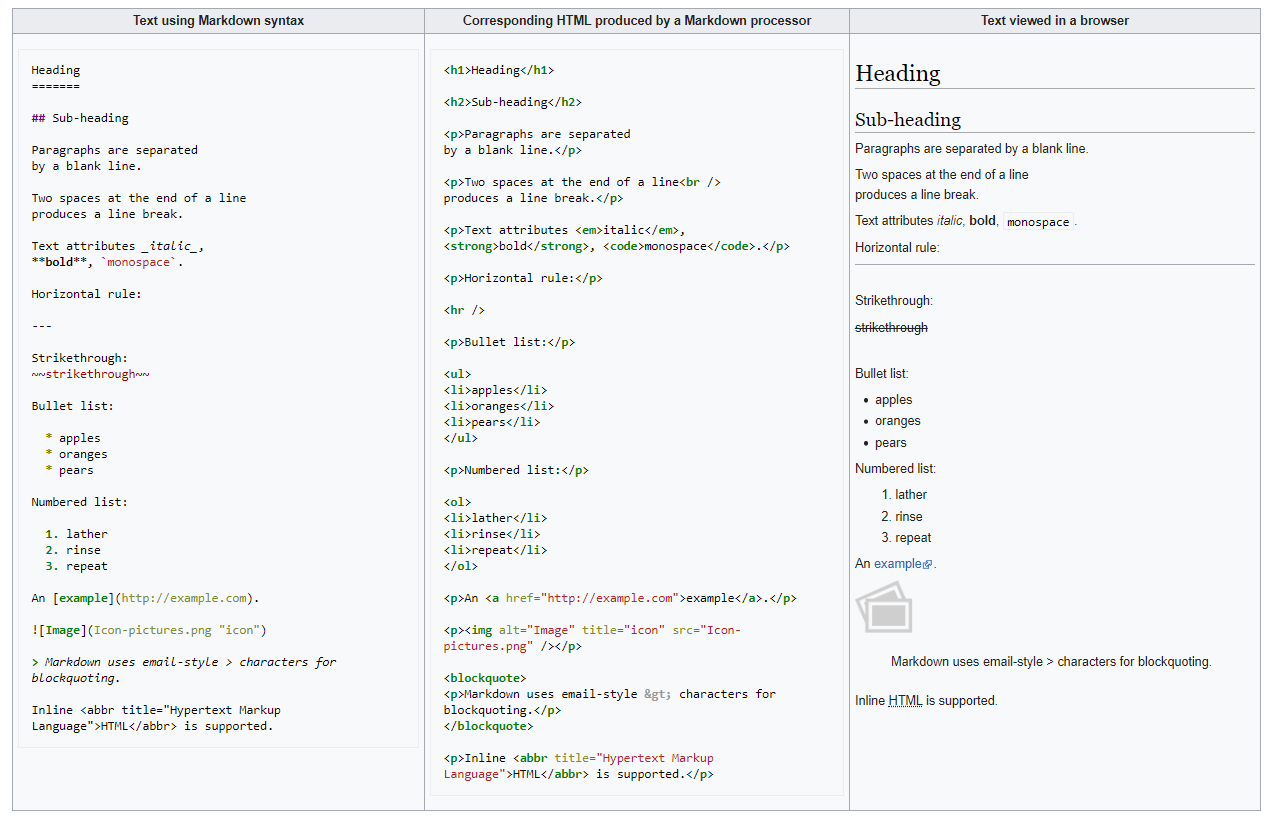
\includegraphics[width=0.8\linewidth]{fig/markdown-http.png}
\end{figure}
* CSP 201703-3
\end{frame}

\begin{frame}{Markdown $\times$ VS Code}
\href{https://github.com/shd101wyy/vscode-markdown-preview-enhanced}{Markdown Preview Enhanced}
\begin{figure}
\centering
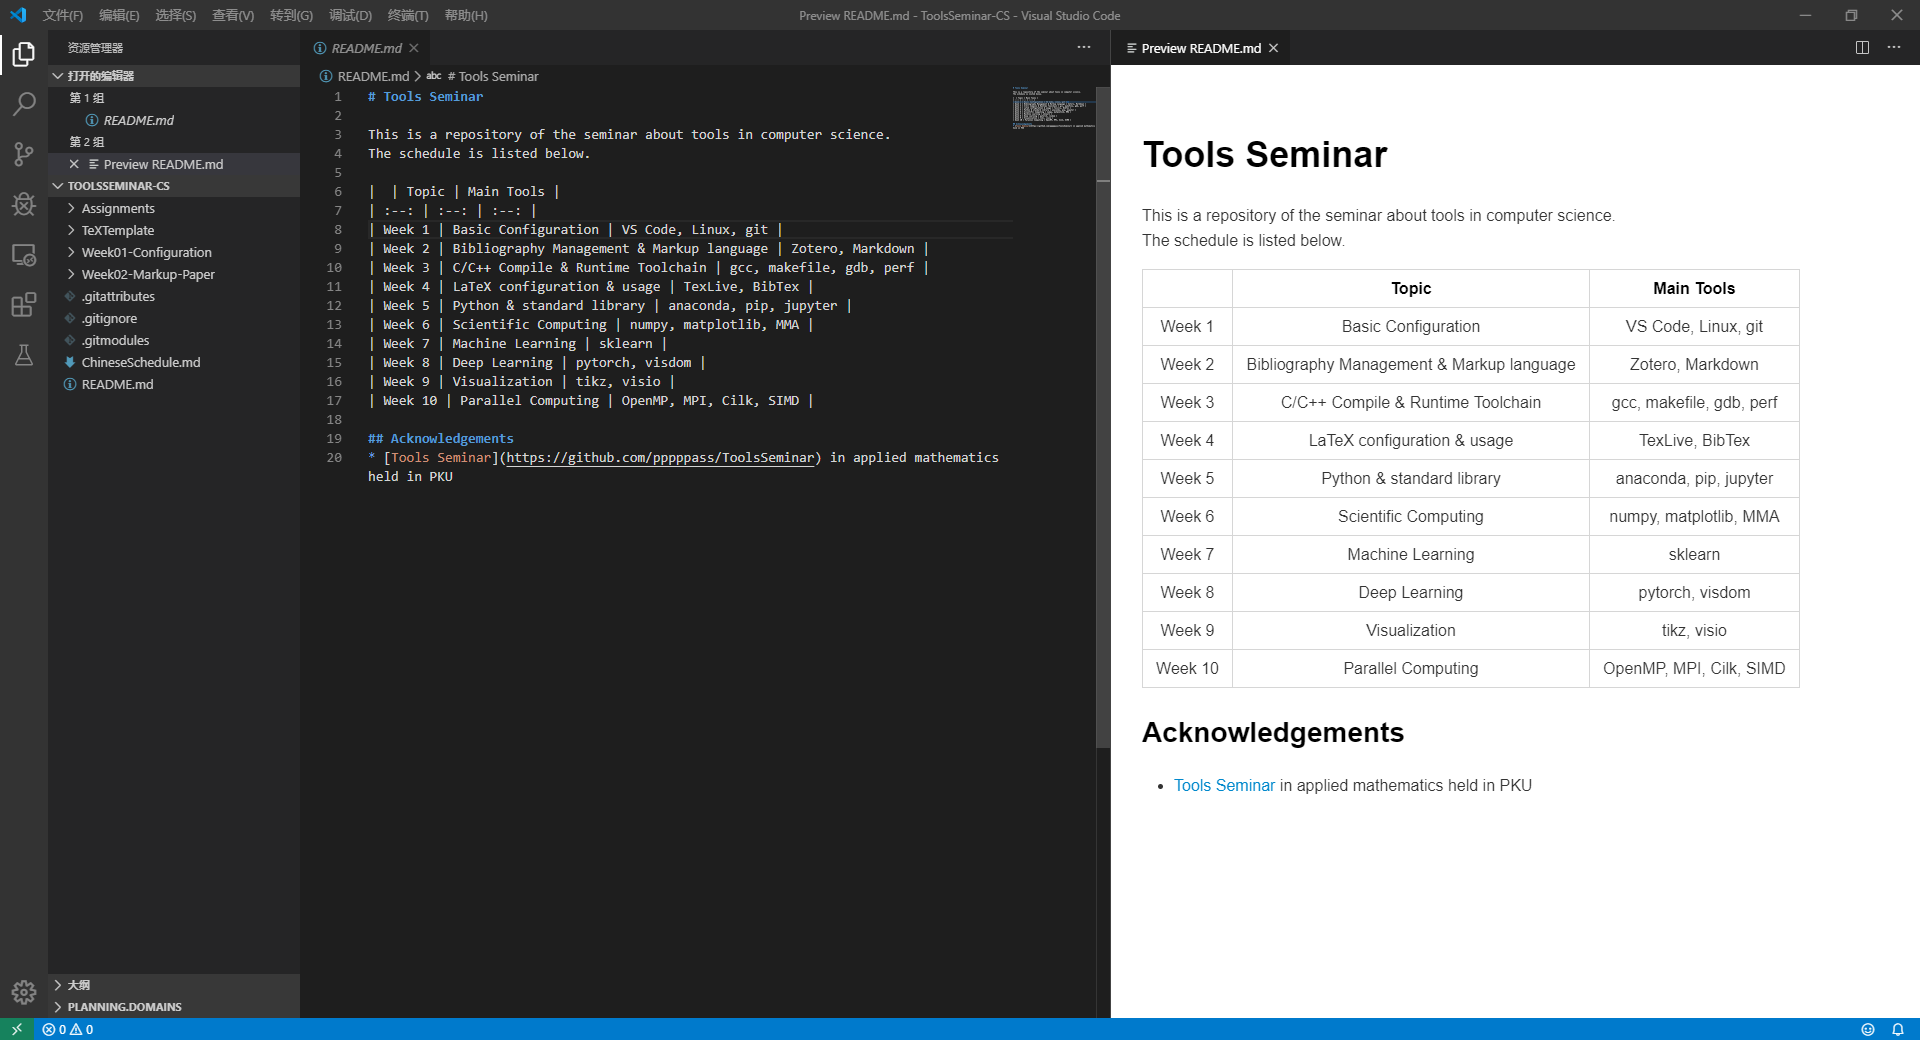
\includegraphics[width=\linewidth]{fig/markdown-preview.png}
\end{figure}
\end{frame}

\section{Scientific Literature}
\begin{frame}
\sectionpage
\end{frame}

\begin{frame}{Official Rankings on CS}
\begin{itemize}
	\item Conference / Journal Ranking: \href{https://www.ccf.org.cn/xspj/gyml/}{China Computer Federation (CCF)}
	\item University Ranking: \href{http://csrankings.org/\#/index?all}{CS Rankings}
\end{itemize}
\end{frame}

\begin{frame}{Top Schools in CS}
CS Ranking by \href{http://csrankings.org/\#/index?all}{CSRankings} (2019.11.19)
\begin{itemize}
	\item Carnegie Mellon University (CMU)
	\item Massachusetts Institute of Technology (MIT)
	\item Univ. of Illinois at Urbana-Champaign (UIUC)
	\item Stanford University
	\item University of California - Berkeley (UCB)
	\item Cornell University
	\item University of Michigan
	\item University of Washington
	\item University of California - San Diego (UCSD)
\end{itemize}
\end{frame}

\begin{frame}{Paper Resources}
All the resources can be accesses with a school IP address
\begin{itemize}
	\item \href{https://ieeexplore.ieee.org/Xplore/home.jsp}{IEEE Xplore} Digital Library
	\item \href{https://dl.acm.org/}{ACM DL} Digital Library
	\item \href{https://arxiv.org/}{arXiv}: Electronic preprints
	\item \href{https://dblp.org/}{dblp}: Computer Science Bibliography
	\item \href{https://scholar.google.com/}{Google Scholar}
\end{itemize}
For CS, conference $>>$ journal
\end{frame}

\begin{frame}{Paper Organization}
Mainly research paper, not survey:
\begin{itemize}
	\item Title, Author list (first, corresponding)
	\item Abstract, Keywords
	\item Introduction
	\item Background \& Motivation
	\item Methodologies
	\item Experiments
	\item Related Work
	\item Conclusions \& Discussions
	\item Acknowledgments
	\item References: Once you use others' points of view / results / conclusions, you MUST cite!
\end{itemize}
* Take TVM [OSDI'18] \& GraphDynS [MICRO'19] paper as examples
\end{frame}

\begin{frame}{Bibliography}
Bib\TeX file:
\begin{itemize}
	\item Title
	\item Authors
	\item Conference / Journal
	\item (Book: publisher, pages)
	\item Year
\end{itemize}
* \emph{Download citations} from ACM/IEEE
\end{frame}

\begin{frame}{Literature Management}
\href{https://www.zotero.org}{Zotero}: collect, organize, cite, and share research
\begin{figure}
\centering
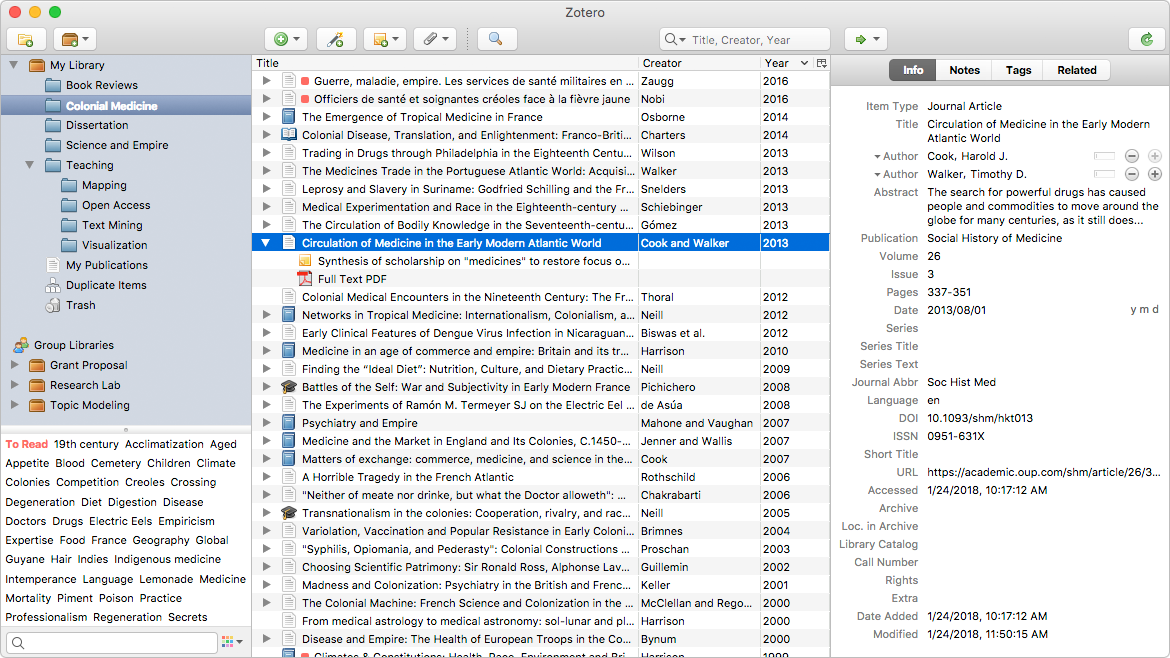
\includegraphics[width=0.8\linewidth]{fig/zotero.png}
\end{figure}
\end{frame}
% A great intro here \url{https://speakerdeck.com/markding/collecting-organizing-and-citing-scientific-literature-an-intro-to-zotero?slide=20}

\begin{frame}{Zotero}
\begin{itemize}
	\item Brower support
	\item Retrieve PDF metadata
	\item Duplicate detection
	\item Generate bibliographies (Bib\TeX)
	\item Sync with your account
\end{itemize}
\end{frame}

\section{Summary}
\begin{frame}
\sectionpage
\end{frame}

\begin{frame}{Week 2 - Markup Languages \& Scientific Literature}
\begin{itemize}
	\item Markup languages: XML, Markdown
	\item CS Ranking
	\item Literature resources: ACM, IEEE, arXiv
	\item Paper organization
	\item Literature management: Zotero
\end{itemize}
\end{frame}

\end{document}